\subsubsection{本走行・実験走行で見つかった課題}
\paragraph{走行不可能領域への侵入でロボットが動作不能になる問題}
むぎまるチームは本走行において, navigation2が経路生成をする際に参照する
コストマップにおける走行不可能領域にロボットが侵入して, 
動作不能に陥ったことでリタイアとなった. 
この状況をRvizを用いて可視化した際の画像を図\ref{fig:mugimaru_result}に示す. 
図中のピンク色の範囲は走行不可能領域のコスト, 
水色の範囲はロボットの内接円半径を考慮した走行不可能領域のコストを表している. 
つまり, ロボットの中心が水色の範囲に侵入すると
ロボットが走行不可能領域にいると判断される. 
%%%中心の話をするなら画像内でも中心を表現したほうが見やすい気がする. 
図\ref{fig:mugimaru_result}からロボットの中心は
水色の範囲に侵入していることが確認できる. 
この状態になると, navigation2は目的地までの経路及び動作を生成しなくなる. 
このようになったとき, リカバリー動作が有効に働かずナビゲーションを中断してしまった. 

この問題への対策として, 走行可能領域に入るまで
障害物を回避しながら動き回るという復帰動作を実装することが
一つ挙げられる. 
図からロボットの前方には走行可能領域があることが確認できる. 
その場所までLiDARにより周囲の障害物を検知して, 
それらを回避しながら移動可能であれば, 
この問題が発生した場合にでもナビゲーションを続行できるようになると考える. 
\begin{figure}[h]
  \begin{center}
  	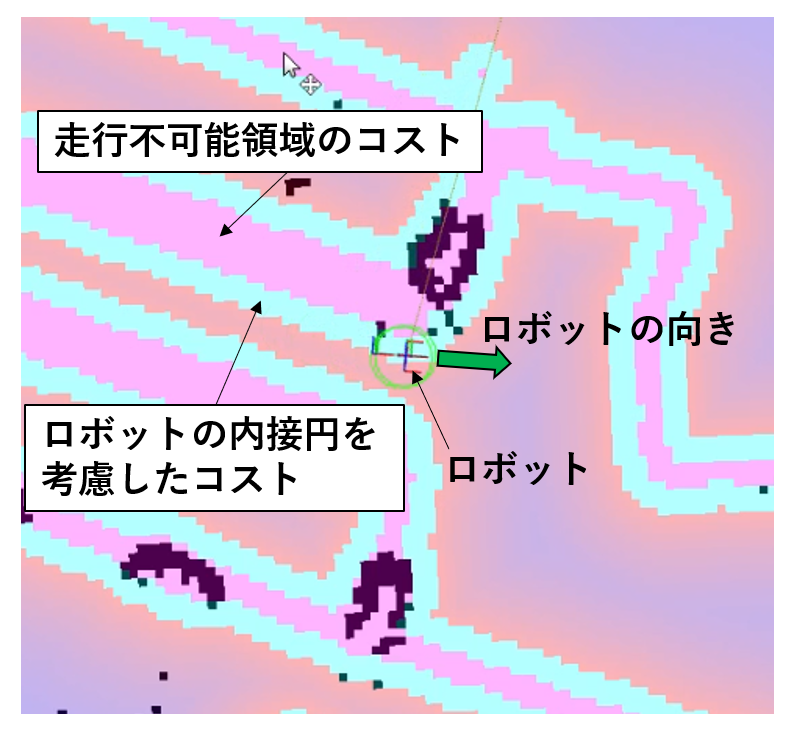
\includegraphics[width=0.9\linewidth]{figs/mugimaru_result.eps}
  	\caption{ロボットがコストマップに乗り上げた状況の図} 
  	\label{fig:mugimaru_result}
  \end{center}
\end{figure}

